\chapterimage{champagne-cross-section-2.jpg} % Chapter heading image

\chapter{O que é um Ponteiro?}
\lstcodestyle
Uma daquelas coisas que os iniciantes em C acham difícil é o conceito de ponteiros. O objetivo deste texto é fornecer uma introdução aos ponteiros e seu uso para esses iniciantes.

Eu descobri que muitas vezes o principal motivo pelo qual os iniciantes têm problemas com ponteiros é que eles têm uma percepção fraca ou mínima das variáveis (como são usadas em C). Assim, começamos com uma discussão das variáveis C em geral.

Uma \textbf{variável} em um programa é algo com um nome, cujo valor pode variar. A maneira como o compilador e o \textit{linker} lidam com isso é que ele atribui um bloco específico de memória dentro do computador para armazenar o valor daquela variável. O tamanho desse bloco depende do intervalo no qual a variável pode variar. Por exemplo, em PCs, o tamanho de uma variável inteira é de 4 bytes e o de um inteiro longo é de 8 bytes. Em C, o tamanho de um tipo de variável, como um inteiro, não precisa ser o mesmo em todos os tipos de máquinas.

Quando declaramos uma variável, informamos ao compilador duas coisas, o nome da variável e o tipo da variável. Por exemplo, declaramos uma variável do tipo inteiro com o nome \textit{k} escrevendo:

\begin{lstlisting}
	int k;
\end{lstlisting}

Ao ver a parte ``int'' dessa instrução, o compilador reserva 4 bytes de memória (em um PC de 32 bits) para armazenar o valor do inteiro. Também configura uma tabela de símbolos. Nessa tabela, ele adiciona o símbolo \textit{k} e o endereço relativo na memória onde esses 4 bytes foram reservados.

Então, se mais tarde escrevermos:
\begin{lstlisting}
	k = 2;
\end{lstlisting}
esperamos que, em tempo de execução quando esta instrução for executada, o valor 2 seja colocado naquele local de memória reservado para o armazenamento do valor de \textbf{k}. Em C, nos referimos a uma variável como o inteiro \textbf{k} como um ``objeto''.

Em certo sentido, existem dois `valores'' associados ao objeto \textbf{k}. Um é o valor do número inteiro armazenado lá (2 no exemplo acima) e o outro é o ``valor'' da localização da memória, ou seja, o endereço de \textbf{k}. Alguns textos referem-se a esses dois valores com a nomenclatura \textbf{\textit{rvalue}} (valor à direita, pronunciado ``ar value'') e \textbf{\textit{lvalue}} (valor à esquerda, pronunciado ``el value''), respectivamente.

Em alguns linguagens, o \textit{lvalue} é o valor permitido no lado esquerdo do operador de atribuição `=' (ou seja, o endereço onde termina o resultado da avaliação do lado direito). O \textit{rvalue} é aquele que está no lado direito da instrução de atribuição, o 2 acima. \textit{Rvalues} não podem ser usados no lado esquerdo da instrução de atribuição. Assim: \textbf{2 = k}; é ilegal.

Na verdade, a definição acima de ``lvalue'' é um pouco modificada para C. De acordo com \textbf{K\&R II} (página 197): \cite{kr}.

\begin{quotation}
	``Um \textbf{objeto} é uma região nomeada de armazenamento; um \textbf{lvalue} é uma expressão que se refere a um objeto''`
\end{quotation}

No entanto, neste ponto, a definição originalmente citada acima é suficiente. À medida que nos familiarizamos com os ponteiros, entraremos em mais detalhes sobre isso.

Ok, agora considere:

\begin{lstlisting}[numbers=left, numberstyle=\tiny]
	int j, k;

	k = 2;
	j = 7; (*@\label{linha1}@*)
	k = j; (*@\label{linha2}@*)
\end{lstlisting}

Acima, o compilador interpreta o \textbf{j} na linha \ref{linha1} como o endereço da variável \textbf{j} (seu \textit{lvalue}) e cria o código para copiar o valor 7 para esse endereço. Na linha \ref{linha2}, entretanto, \textbf{j} é interpretado como seu \textit{rvalue} (uma vez que está no lado direito do operador de atribuição '='). Ou seja, aqui \textbf{j} se refere ao valor armazenado no local da memória reservado para \textbf{j}, neste caso 7. Assim, o 7 é copiado para o endereço designado pelo \textit{lvalor} de \textbf{k}.

Em todos esses exemplos, estamos usando inteiros de 4 bytes, portanto, todas as cópias de \textit{rvalues} de um local de armazenamento para o outro são feitas copiando 4 bytes. Se estivéssemos usando números inteiros longos, estaríamos copiando 8 bytes.

Agora, digamos que temos um motivo para querer uma variável projetada para conter um \textit{lvalue} (um endereço). O tamanho necessário para armazenar tal valor depende do sistema. Em computadores de mesa mais antigos com 64 K de memória total, o endereço de qualquer ponto da memória pode estar contido em 2 bytes. Os computadores com mais memória exigiriam mais bytes para armazenar um endereço. O tamanho real necessário não é muito importante, desde que tenhamos uma maneira de informar ao compilador que o que queremos armazenar é um endereço.

Essa variável é chamada de \textbf{ponteiro} (por razões que, esperamos, ficarão mais claras um pouco mais tarde). Em C, quando definimos uma variável como ponteiro, fazemos isso precedendo seu nome com um asterisco. Em C, também damos ao nosso ponteiro um tipo que, neste caso, se refere ao tipo de dados armazenados no endereço que iremos armazenar em nosso ponteiro. Por exemplo, considere a declaração da variável:

\begin{lstlisting}
	int *ptr;
\end{lstlisting}

\textbf{ptr} é o nome da nossa variável (assim como \textbf{k} era o nome da nossa variável inteira). O `*' informa ao compilador que queremos uma variável de ponteiro, ou seja, separar quantos bytes forem necessários para armazenar um endereço na memória. O \textbf{int} diz que pretendemos usar nossa variável de ponteiro para armazenar o endereço de um inteiro. Diz-se que esse ponteiro ``aponta para'' um número inteiro. No entanto, observe que quando escrevemos \textbf{int k;} não atribuímos um valor a \textbf{k}. Se essa definição for feita fora de qualquer função, os compiladores compatíveis com ANSI irão inicializá-la com zero. Da mesma forma, \textbf{ptr} não tem valor, ou seja, não armazenamos um endereço nele na declaração acima. Nesse caso, novamente se a declaração estiver fora de qualquer função, ela é inicializada com um valor garantido de forma que não aponte para nenhum objeto ou função C. Um ponteiro inicializado dessa maneira é chamado de ponteiro ``nulo''.

O padrão de bits real usado para um ponteiro nulo pode ou não ser avaliado como zero, pois depende do sistema específico no qual o código é desenvolvido. Para tornar o código-fonte compatível entre vários compiladores em vários sistemas, uma macro é usada para representar um ponteiro nulo. Essa macro é chamada de \textbf{NULL}. Portanto, definir o valor de um ponteiro usando a macro \textbf{NULL}, como em uma instrução de atribuição como \textbf{ptr = NULL}, garante que o ponteiro se tornou um ponteiro nulo. Da mesma forma, assim como se pode testar um valor inteiro igual a zero, como em \textbf{if (k == 0)}, podemos testar um ponteiro nulo usando \textbf{if (ptr == NULL)}.

Mas, de volta ao uso de nossa nova variável \textbf{ptr}. Suponha agora que queremos armazenar em \textbf{ptr} o endereço de nossa variável inteira \textbf{k}. Para fazer isso, usamos o operador \textbf{\&} unário e escrevemos:

\begin{lstlisting}
	ptr = &k;
\end{lstlisting}

O que o operador \textbf{\&} faz é recuperar o \textit{lvalue} (endereço) de \textbf{k}, embora \textbf{k} esteja no lado direito do operador de atribuição `=', e o copia para o conteúdo do nosso ponteiro \textbf{ptr}. Agora, diz-se que \textbf{ptr} ``aponta para'' \textbf{k}. Tenha paciência conosco agora, há apenas mais um operador que precisamos discutir.

O ``operador de desreferenciação'' é o asterisco e é usado da seguinte forma:

\begin{lstlisting}
	*ptr = 7;
\end{lstlisting}
irá copiar 7 para o endereço apontado por \textbf{ptr}. Assim, se \textbf{ptr} ``aponta para'' (contém o endereço de) \textbf{k}, a instrução acima irá definir o valor de \textbf{k} para 7. Ou seja, quando usamos o `*' desta forma estamos nos referindo ao valor para o qual \textbf{ptr} está apontando, não o valor do próprio ponteiro.

Da mesma forma, poderíamos escrever:
\begin{lstlisting}
	printf("%d\n",*ptr);
\end{lstlisting}
para imprimir na tela o valor inteiro armazenado no endereço apontado por \textbf{ptr;}.

Uma maneira de ver como tudo isso se encaixa seria executar o programa a seguir e, em seguida, revisar o código e a saída com cuidado.

\lstinputlisting[label={prog1-1}, caption={Variáveis e ponteiros}, numbers=left, numberstyle=\tiny, stepnumber=1]{code/prog1-1.c}

O programa \ref{prog1-1} foi compilado com o compilador gnu gcc, com as seguintes opções:\\
\lstconsolestyle
\begin{lstlisting}
	gcc -Wall -std=c11 -pedantic -o prog1-1 prog1-1.c	
\end{lstlisting}

O parâmetro \texttt{Wall} faz com que o compilador emita todos os \textit{warnings}; \texttt{-std=c11} diz que ele deve seguir a versão \textbf{c11} da linguagem; e finalmente, \texttt{-pedantic} diz que ele deve seguir estritamente o padrão da linguagem, ignorando possíveis extensões do compilador.

Um resultado possível, executando em um computador de 64 bits, seria:
\lstconsolestyle
\begin{lstlisting}
j tem valor 1 e está armazenado em 0x562dcb413018
k tem valor 2 e está armazenado em 0x562dcb413028
ptr tem valor 0x562dcb413028 e está armazenado em 0x562dcb413020
O valor do inteiro apontado por ptr é 2
\end{lstlisting}
\lstcodestyle
\begin{remark}
	Ainda temos que discutir os aspectos de C que requerem o uso da expressão \textbf{(void *)} para fazer a conversão de ponteiros para \textbf{int} para ponteiros para \textbf{void}, necessárias aqui para a impressão com \textbf{\%p}. Por enquanto, ignoramos este aspecto e nosso código é compilado com a opção \texttt{-pedantic}, que causa diversos \textit{warnings} caso não seja feita a conversão com \textbf{(void*)}. Voltaremos a este assunto na Seção \ref{expvoid}.

\end{remark}

A Figura \ref{enderecos} representa esquematicamente a memória para este arranjo de variáveis. Lembre-se que neste caso estamos trabalhando com um computador de 64 bits, assim os endereços têm 8 bytes (dos quais escrevemos 6, por simplicidade). 

\begin{figure}[ht]
	\begin{center}
		% Graphic for TeX using PGF
% Title: /home/araujo/Dropbox/VerbTeX/LivroComputadores/Pictures/memoria.dia
% Creator: Dia v0.97.3
% CreationDate: Sun May 21 11:59:17 2017
% For: araujo
% \usepackage{tikz}
% The following commands are not supported in PSTricks at present
% We define them conditionally, so when they are implemented,
% this pgf file will use them.
\ifx\du\undefined
  \newlength{\du}
\fi
\setlength{\du}{15\unitlength}
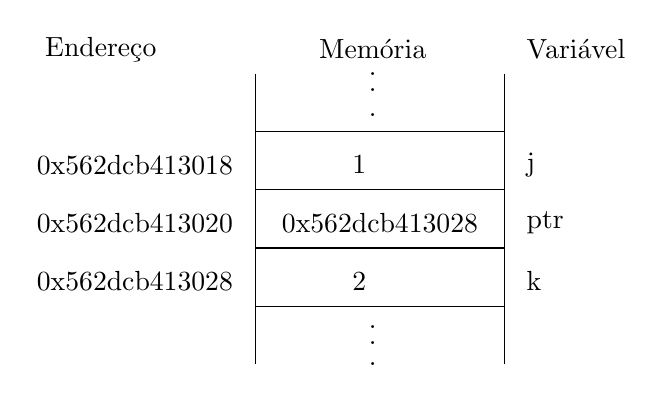
\begin{tikzpicture}
\pgftransformxscale{1.000000}
\pgftransformyscale{-1.000000}
\definecolor{dialinecolor}{rgb}{0.000000, 0.000000, 0.000000}
\pgfsetstrokecolor{dialinecolor}
\definecolor{dialinecolor}{rgb}{1.000000, 1.000000, 1.000000}
\pgfsetfillcolor{dialinecolor}

\draw (31\du,9.4\du)--(31.\du,8\du)--(25\du,8\du)--(25\du,9.4\du);
\node at (27.5\du,8.8\du){1};
\draw (31\du,10.8\du)--(31.\du,9.4\du)--(25\du,9.4\du)--(25\du,10.8\du);
\node at (28\du,10.2\du){0x562dcb413028};
\draw (31\du,12.2\du)--(31.\du,10.8\du)--(25\du,10.8\du)--(25\du,12.2\du);
\node at (27.5\du,11.6\du){2};
\draw (31\du,13.6\du)--(31.\du,12.2\du)--(25\du,12.2\du)--(25\du,13.6\du);
%\node at (27.5\du,13\du){0110 0100};
%\draw (31\du,15\du)--(31.\du,13.6\du)--(25\du,13.6\du)--(25\du,15\du);
%\node at (27.5\du,14.4\du){0110 1100};
%\draw (31\du,16.4\du)--(31.\du,15\du)--(25\du,15\du)--(25\du,16.4\du);
%\node at (27.5\du,15.8\du){0110 1111};
%\draw (31\du,17.8\du)--(31.\du,16.4\du)--(25\du,16.4\du)--(25\du,17.8\du);
%\node at (27.5\du,17.2\du){0110 1100};
%\draw (31\du,17.8\du)--(31.\du,16.4\du)--(25\du,16.4\du)--(25\du,17.8\du);
%\node at (27.5\du,18.6\du){0110 1100};
%\draw (31\du,19.2\du)--(31.\du,17.8\du)--(25\du,17.8\du)--(25\du,19.2\du)--cycle;
\node[anchor=west] at (27.5\du,12.7\du){.};
\node[anchor=west] at (27.5\du,13.100000\du){.};
\node[anchor=west] at (27.5\du,13.600000\du){.};

\definecolor{dialinecolor}{rgb}{0.000000, 0.000000, 0.000000}
\pgfsetstrokecolor{dialinecolor}
%\draw (25\du,19.2\du)--(25\du,20.6\du);
%\draw (31\du,19.2\du)--(31\du,20.6\du);
\draw (25\du,6.6\du)--(25\du,8\du);
\draw (31\du,6.6\du)--(31\du,8\du);
\node[anchor=west] at (27.5\du,7.600000\du){.};
\node[anchor=west] at (27.5\du,7.000000\du){.};
\node[anchor=west] at (27.5\du,6.600000\du){.};
\node[anchor=west] at (19.5\du,8.8\du){0x562dcb413018};
\node[anchor=west] at (19.5\du,10.2\du){0x562dcb413020};
\node[anchor=west] at (19.5\du,11.6\du){0x562dcb413028};
%\node[anchor=west] at (19.5\du,13\du){1204};
%\node[anchor=west] at (19.5\du,14.4\du){1205};
%\node[anchor=west] at (19.5\du,15.8\du){1206};
%\node[anchor=west] at (19.5\du,17.2\du){1207};
%\node[anchor=west] at (19.5\du,18.4\du){1208};
\node[anchor=west] at (19.7\du,6.002347\du) {Endere\c{c}o};
\node[anchor=west] at (26.3\du,6.002347\du){Mem\'{o}ria};
\node[anchor=west] at (31.3\du,6.002347\du){Vari\'{a}vel};
\node[anchor=west] at (31.3\du,8.8\du){j};
\node[anchor=west] at (31.3\du,10.2\du){ptr};
\node[anchor=west] at (31.3\du,11.6\du){k};
\end{tikzpicture}

		\caption{Endereços e memória.}
		\label{fig:esquemamemoria}
	\end{center}
\label{enderecos}
\end{figure}


\section*{Para revisar:}
\begin{itemize}
	\item Uma variável é declarada dando-lhe um tipo e um nome (por exemplo, \textbf{int k;})
	\item Uma variável de ponteiro é declarada dando a ela um tipo e um nome (por exemplo, \textbf{int * ptr}) onde o asterisco diz ao compilador que a variável chamada \textbf{ptr} é uma variável de ponteiro e o tipo diz ao compilador para qual tipo o ponteiro deve apontar (inteiro nesse caso).
	\item Uma vez que uma variável é declarada, podemos obter seu endereço precedendo seu nome com o operador unário \textbf{\&}, como em \textbf{\&k}.
	\item Podemos ``desreferenciar'' um ponteiro, ou seja, referir-se ao valor para o qual ele aponta, usando o operador unário `*' como em \textbf{*ptr}.
	\item Um ``\textit{lvalue}'' de uma variável é o valor do seu endereço, ou seja, onde está armazenado na memória. O ``\textit{rvalue}'' de uma variável é o valor armazenado nessa variável (naquele endereço).
\end{itemize}

